\chapter{Specyfikacja wewnętrzna}
\label{ch:05}


Jeśli „Specyfikacja wewnętrzna”:
\begin{itemize}
\item przedstawienie idei
\item architektura systemu
\item opis struktur danych (i organizacji baz danych)
\item komponenty, moduły, biblioteki, przegląd ważniejszych klas (jeśli występują)
\item przegląd ważniejszych algorytmów (jeśli występują)
\item szczegóły implementacji wybranych fragmentów, zastosowane wzorce projektowe
\item diagramy UML
\end{itemize}

% % % % % % % % % % % % % % % % % % % % % % % % % % % % % % % % % % % 
% Pakiet minted wymaga importu: \usepackage{minted}                 %
% i specjalnego kompilowania:                                       %
% pdflatex -shell-escape main                                       %
% % % % % % % % % % % % % % % % % % % % % % % % % % % % % % % % % % % 
Aplikacja Infektosym jest narzędziem symulacyjnym, które zostało stworzone z myślą o zrozumieniu i analizie rozprzestrzeniania się zarażeń w przestrzeni biurowej. Głównym celem projektu jest dostarczenie interaktywnej platformy umożliwiającej obserwację, analizę oraz testowanie scenariuszy związanych z potencjalnymi wirusowymi infekcjami w środowisku pracy.

\begin{itemize}
	\item \textbf{Cele Projektu:}
	\begin{itemize}
		\item Zapewnienie realistycznego modelu symulacji, uwzględniającego codzienne zachowania ludzkie w biurze.
		\item Możliwość dostosowywania parametrów symulacji, takich jak dystans zarażenia, czas do zarażenia czy skuteczność maseczek.
		\item Wizualizacja procesu rozprzestrzeniania się patogenów w czasie rzeczywistym.
	\end{itemize}
	\item \textbf{Koncepcje i Założenia:}
	\begin{itemize}
		\item Implementacja agentowego podejścia, gdzie każdy osobnik w symulacji podejmuje indywidualne decyzje i reaguje na otoczenie.
		\item Duża parametryzacja symulacji, umożliwiająca dostosowanie scenariuszy do różnych warunków i kontekstów.
	\end{itemize}
	\item \textbf{Kierunki Rozwoju:}
	\begin{itemize}
		\item Wprowadzenie zaawansowanych funkcji interakcji między agentami, uwzględniających bardziej złożone scenariusze zachowań.
		\item Integracja z danymi epidemiologicznymi dla bardziej precyzyjnych analiz i prognoz.
		\item Dalsza optymalizacja interfejsu użytkownika i dostępność na różnych platformach.
		\item Wprowadzenie innych scenariuszy np. Szpital, Osiedle, Centrum Handlowe.
	\end{itemize}
\end{itemize}

\section{\textbf{Architektura systemu}}

Architektura systemu aplikacji opiera się na modularnym podejściu, skupiającym się na kilku kluczowych skryptach odpowiedzialnych za różne aspekty symulacji.

\begin{itemize}
	\item \textbf{InterfaceScript:}
	\begin{itemize}
		\item Odpowiada za interakcję z użytkownikiem, umożliwiając mu dostosowywanie parametrów symulacji za pomocą sliderów.
		\item Obsługuje przyciski kontroli, takie jak start, pauza, restart, co zapewnia płynną kontrolę nad symulacją.
		\item Wyświetla istotne statystyki dotyczące aktualnego stanu symulacji, umożliwiając użytkownikowi bieżącą analizę danych.
	\end{itemize}
	
	\item \textbf{GlobalClockScript:}
	\begin{itemize}
		\item Pełni rolę zegara w aplikacji, monitorując czas zarówno w skali symulacji, jak i rzeczywistości.
		\item Liczy dni, godziny oraz ilość godzin symulacji od jej rozpoczęcia, co pozwala na śledzenie postępu w czasie.
		\item Zapewnia synchronizację między symulacją a realnym czasem, co jest istotne dla precyzyjnego odwzorowania dynamiki zarażeń.
	\end{itemize}
	
	\item \textbf{HumanSpawner:}
	\begin{itemize}
		\item Inicjalizuje agentów (ludzi) na mapie, ustawiając je zgodnie z parametrami otrzymanymi od InterfaceScript podczas rozpoczęcia symulacji.
		\item Zapewnia jednolite warunki startowe dla agentów, co umożliwia kontrolowaną analizę scenariuszy symulacyjnych.
	\end{itemize}
	
	\item \textbf{HumanScript:}
	\begin{itemize}
		\item Stanowi rdzeń symulacji zachowań ludzkich, przypisany do każdego obiektu reprezentującego osobę na mapie.
		\item Monitoruje kolizje i stosuje algorytmy określające, czy dany osobnik powinien być narażony na ryzyko zarażenia czy też jest już zainfekowany.
		\item Umożliwia kompleksową symulację interakcji między ludźmi i symulowanie ich zachowań.
	\end{itemize}
	
	\item \textbf{SeatScript:}
	\begin{itemize}
		\item Prosty skrypt odpowiedzialny za zarządzanie miejscami siedzącymi, informując, czy dane miejsce jest zajęte czy wolne.
	\end{itemize}
\end{itemize}

\begin{figure}[h!]
	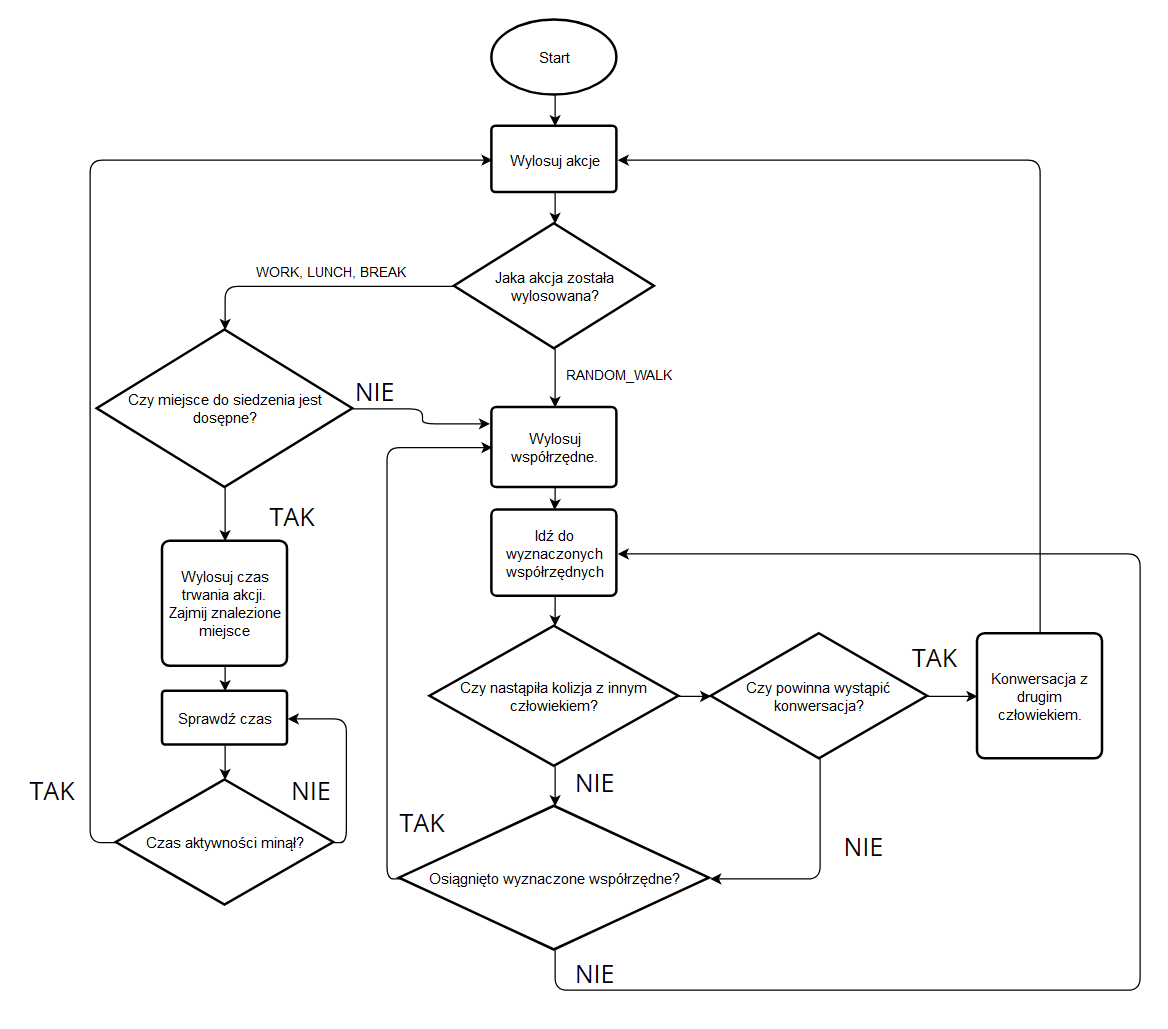
\includegraphics[width=\linewidth]{DiagramAlgorytmuZachowania.png}
	\caption{Sekwencyjny diagram algorytmu symulacji zachowań ludzkich}
\end{figure}


%Krótka wstawka kodu w linii tekstu jest możliwa, np.  \lstinline|int a;| (biblioteka \texttt{listings})% lub  \mintinline{C++}|int a;| (biblioteka \texttt{minted})
%. 
%Dłuższe fragmenty lepiej jest umieszczać jako rysunek, np. kod na rys \ref{fig:pseudokod:listings}% i rys. \ref{fig:pseudokod:minted}
%, a naprawdę długie fragmenty – w załączniku.


%\begin{figure}
%\centering
%\begin{lstlisting}
%class test : public basic
%{
%    public:
%      test (int a);
%      friend std::ostream operator<<(std::ostream & s, 
%                                     const test & t);
%    protected:
%      int _a;  
%     
%};
%\end{lstlisting}
%\caption{Pseudokod w \texttt{listings}.}
%\label{fig:pseudokod:listings}
%\end{figure}

%\begin{figure}
%\centering
%\begin{minted}[linenos,frame=lines]{c++}
%class test : public basic
%{
%    public:
%      test (int a);
%      friend std::ostream operator<<(std::ostream & s, 
%                                     const test & t);
%    protected:
%      int _a;  
%      
%};
%\end{minted}
%\caption{Pseudokod w \texttt{minted}.}
%\label{fig:pseudokod:minted}
%\end{figure}


